\block{\begin{blockbody}\section{Determinants of participant retention for further training}
			\tfont
            Participants' enjoyment of the introductory workshop is strongly linked to how difficult they found it (below left). More importantly, this assigned difficulty level is the key determinant in participants' enthusiasm for further training (below right).\par
            \vms\vms
           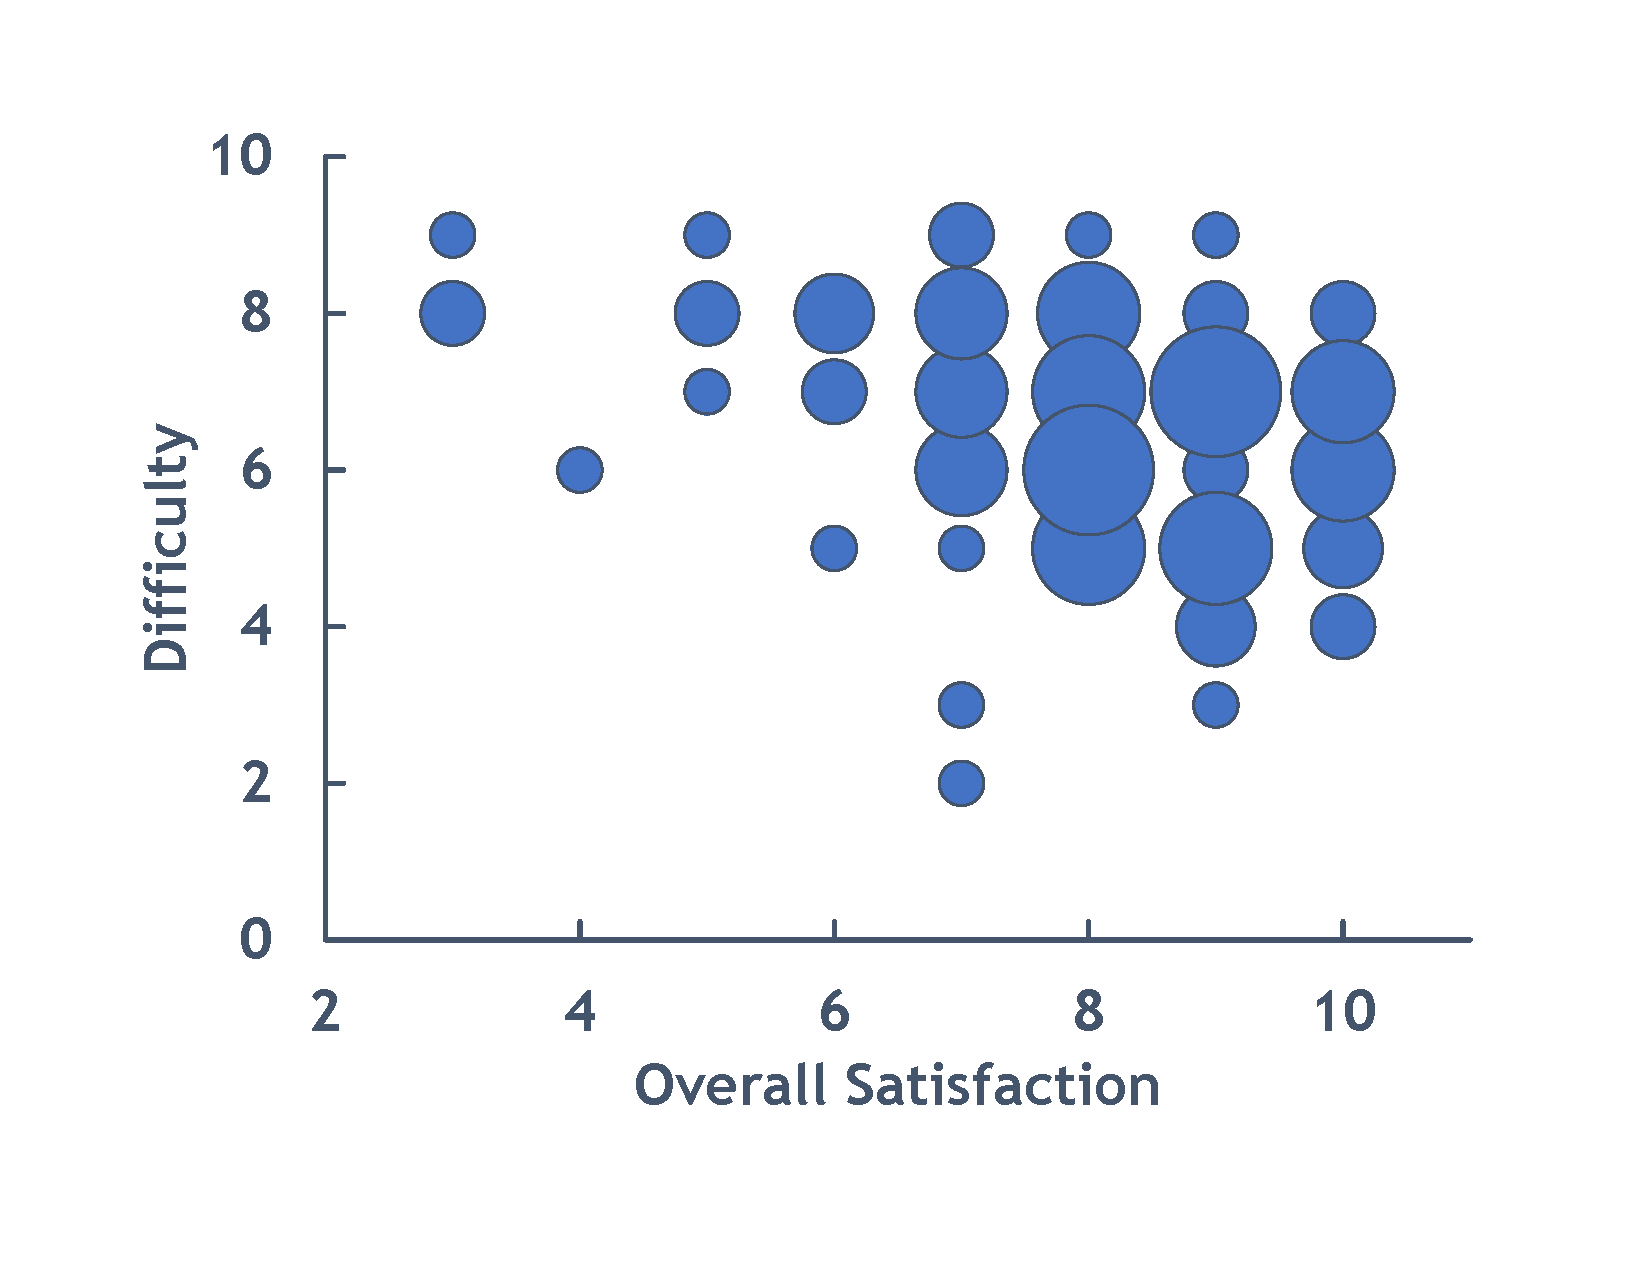
\includegraphics[width = 0.49\textwidth]{OverallVDifficulty}\hfill 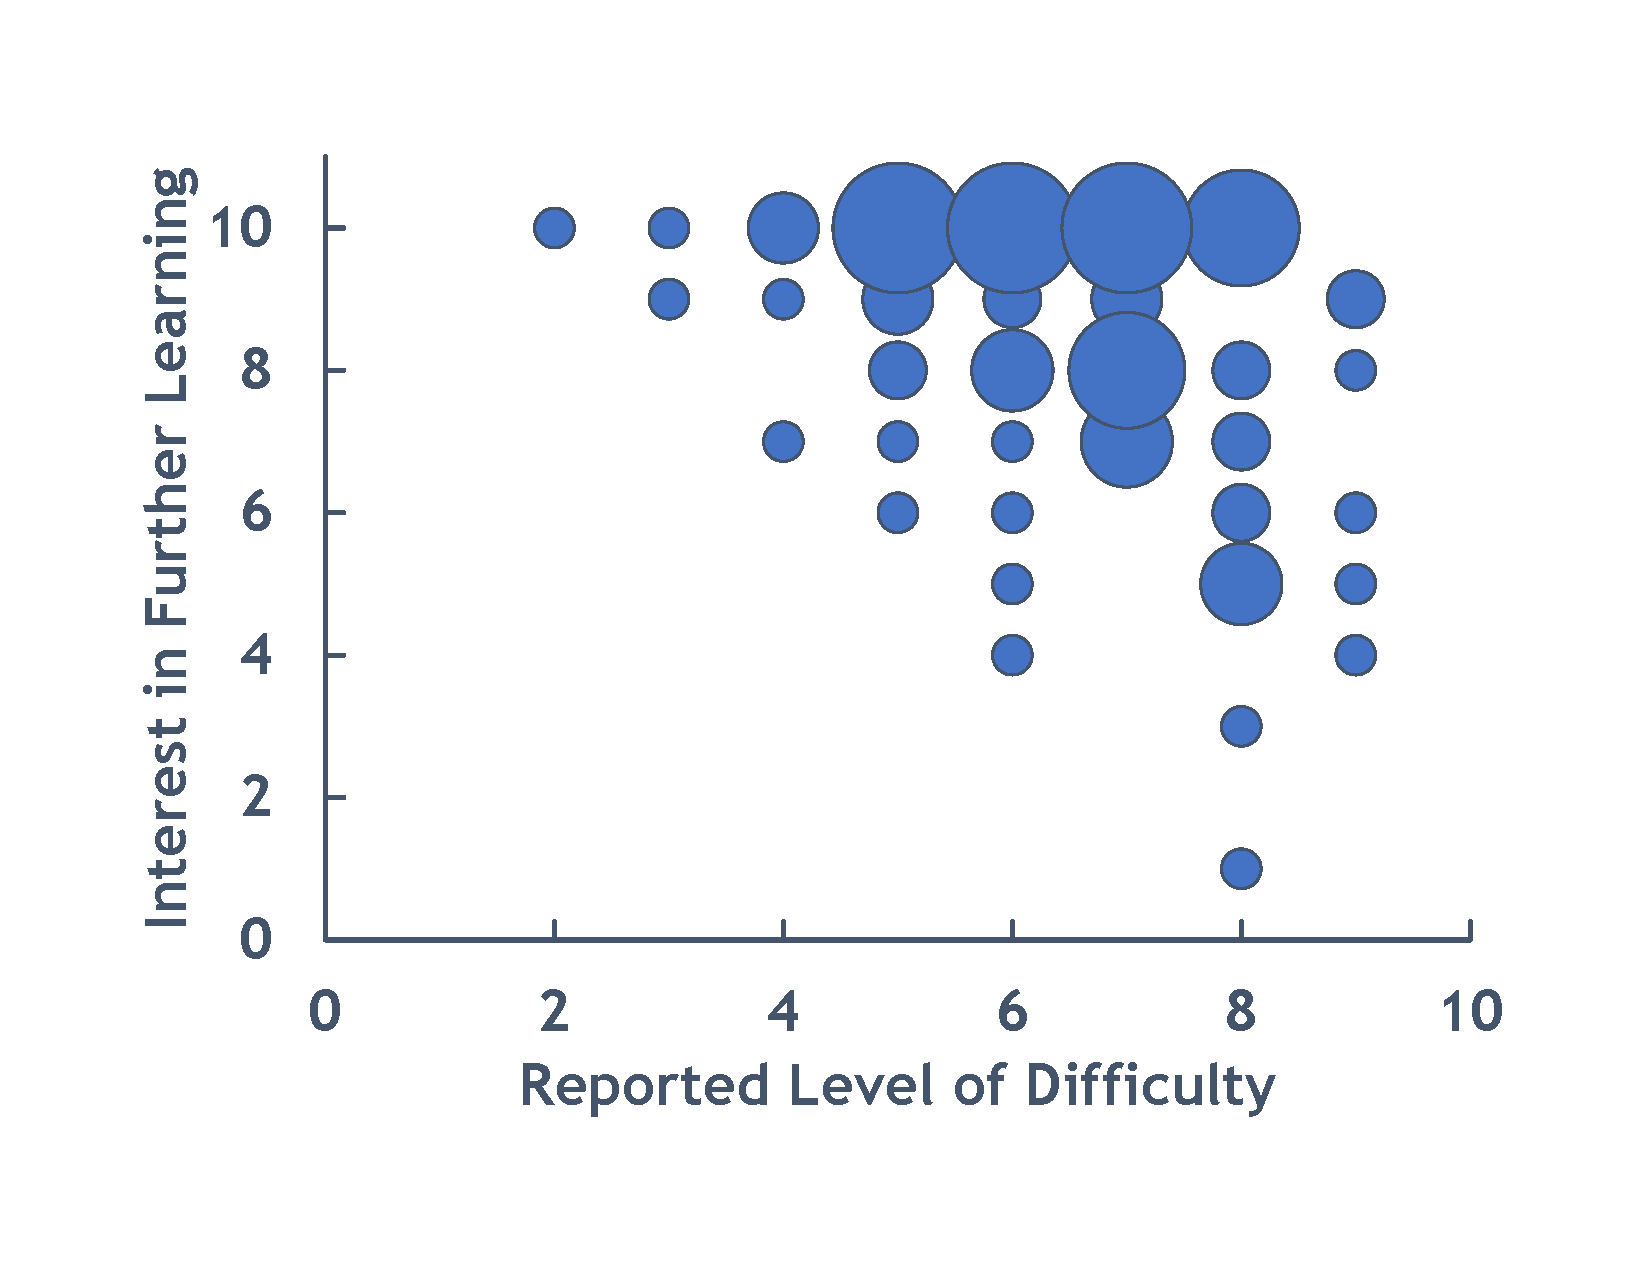
\includegraphics[width = 0.49\textwidth]{DifficultyVFurtherLearning}\par
           \vms\vms\vms\vms\vms
           \begin{minipage}{0.49\textwidth}
           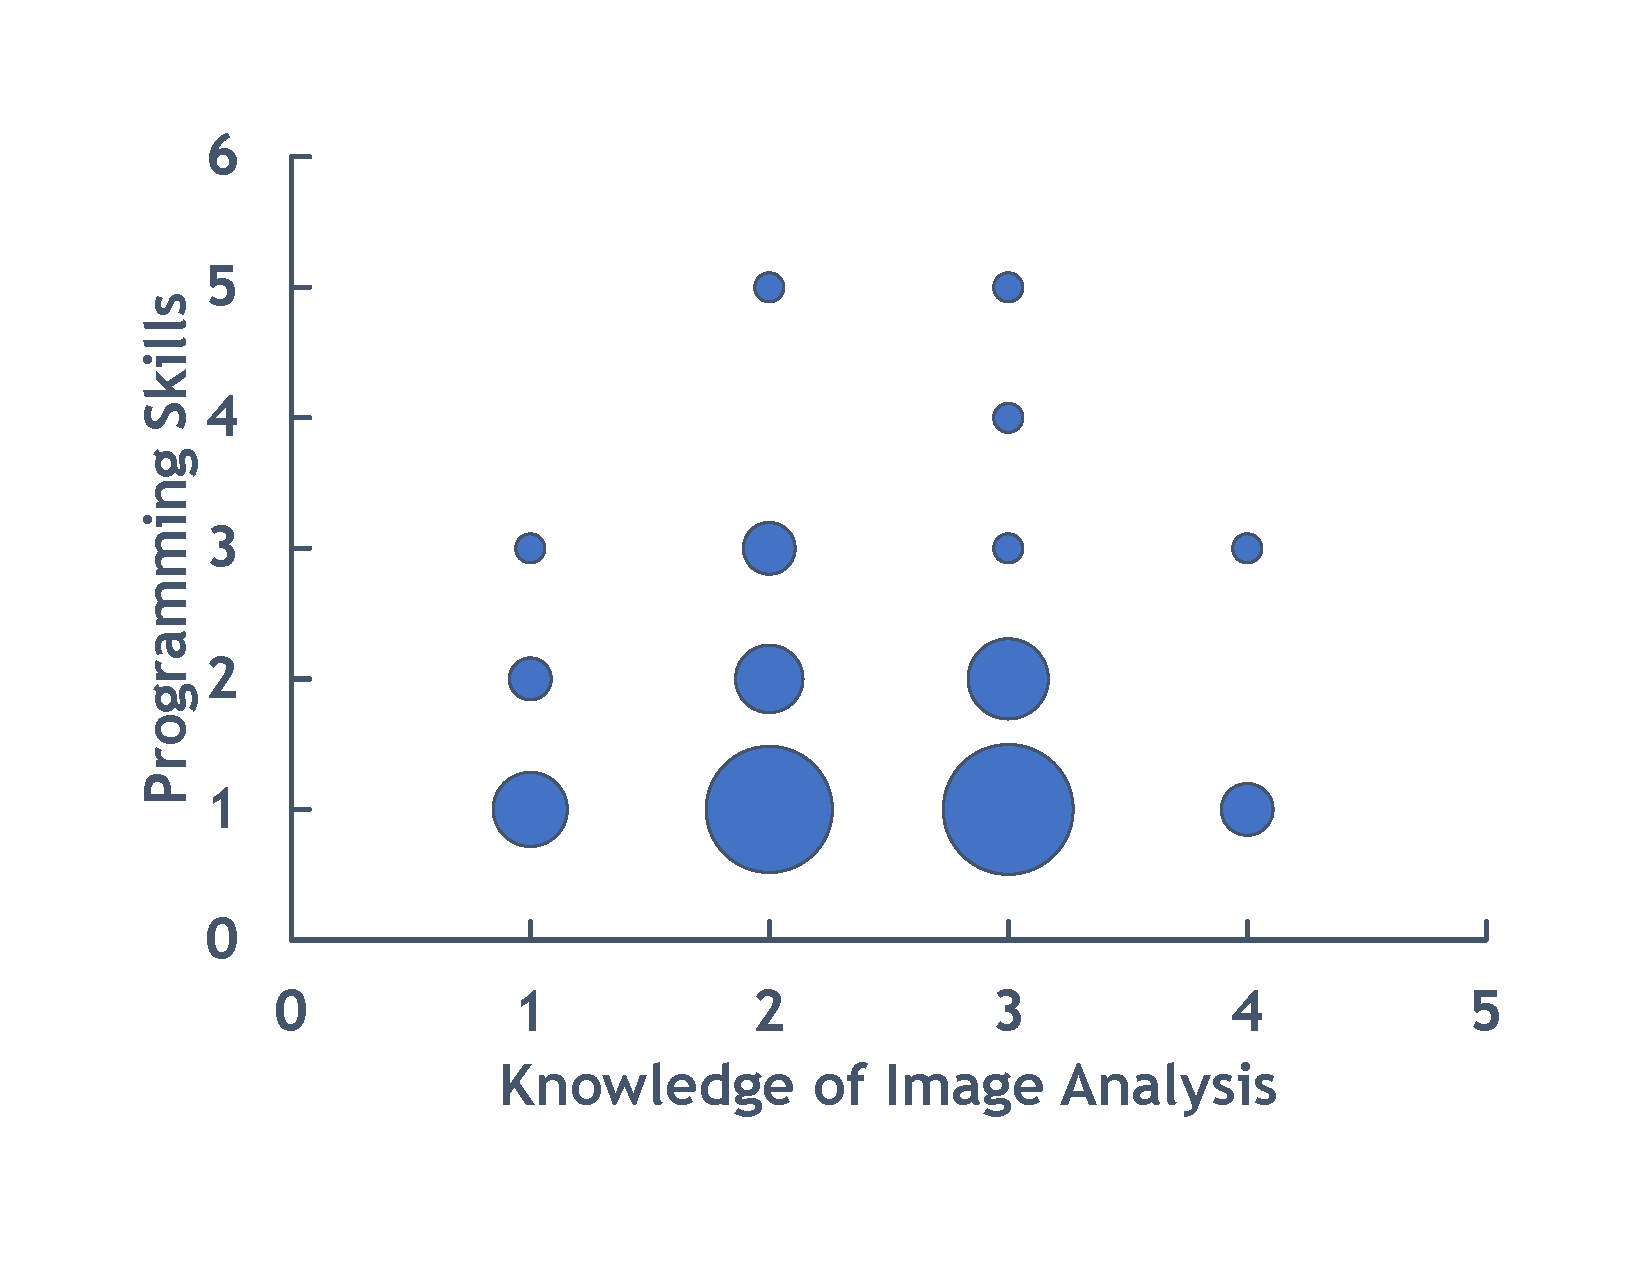
\includegraphics[width = \textwidth]{IAvProgramming}\par
          	\end{minipage} \hfill
            \begin{minipage}{0.49\textwidth}
           It could be considered encouraging that, following our introductory course, many researchers at The Crick now considered themselves to be rather knowledgeable on the subject of image analysis (left). However, given the very short nature of the course and their apparent lack of programming skills, their self-reported knowledge is very likely being overstated. This phenomenon has also been reported elsewhere \citep{Cardona2012}.\par
           \end{minipage}\par
           \vms\vms
           Nevertheless, we are keen to build on the enthusiasm that this introductory course has generated. Taking advantage of the reported interest in further training and with the long-term goal of developing a network of analysts in mind, we have recently begun delivering scripting workshops to address this deficiency in programming skills.\par
		\end{blockbody}}